\section{Resultados}\label{sec:resultados}

\subsection{Configuração experimental}

Executamos a grade completa de hiperparâmetros (Seção~\ref{sec:protocolo}) sobre $\approx$400 reviews IMDb balanceadas (200/classe), split estratificado 70/30, truncamento em 256 tokens.\footnote{Código e dados reprodutíveis: \url{https://github.com/thiago-ouverney/svd-leverage-token-compression}.}
\begin{itemize}
    \item \textbf{Unidade experimental}: cada review como matriz $F \in \mathbb{R}^{T \times D}$ (Seção~\ref{sec:svd-por-documento}); $\bar{T}\approx 209$ linhas após remoção de tokens especiais.
    \item \textbf{Avaliação downstream}: Ridge binário ($\lambda=1$) sobre pooling médio e normalização $L_2$ (Seção~\ref{sec:protocolo-clf}); mede se a seleção algébrica de linhas preserva sinal supervisionado.
    \item \textbf{Referência}: \texttt{full}, sem poda, como baseline sem compressão.
\end{itemize}

\subsection{Diagnóstico espectral: efeito de $\varepsilon$}

Observa-se na curva de energia acumulada (Figura~\ref{fig:epsilon-k}) que parte da energia de $F$ concentra-se nos primeiros modos singulares. Com o aumento de $\varepsilon$, o subespaço dominante ganha dimensão: $\bar{k}$ passa de 34,1 para 50,1 e 92,4 para $\varepsilon=0{,}90$, $0{,}95$ e $0{,}99$ (Tabela~\ref{tab:metricas-eps}).

Dois papéis distintos aparecem no operador:
\begin{itemize}
    \item \textbf{$\varepsilon$}: controla a dimensão do subespaço usado para calcular os leverage scores.
    \item \textbf{$\rho$}: controla quantas linhas são mantidas após o ranqueamento.
\end{itemize}
Tem-se como evidência de que $E_k^{\mathrm{energia}}$, $\bar{R}_k$ e $\bar{k}$ variam com $\varepsilon$ e permanecem invariantes a $\rho$ dentro de cada limiar: essas métricas caracterizam o subespaço truncado $F_k$, e não a seleção final $S$.

\begin{figure}[ht]
    \centering
    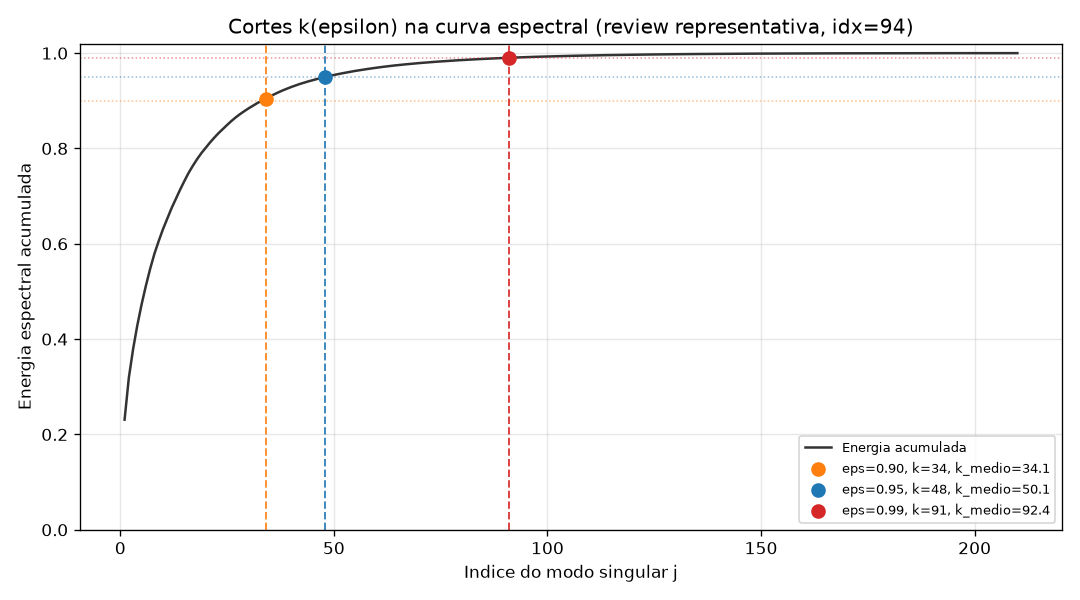
\includegraphics[width=0.92\linewidth]{figures/epsilon_k_cortes.png}
    \caption{Energia espectral acumulada de uma review representativa e pontos de corte $k(\varepsilon)$ para $\varepsilon \in \{0{,}90, 0{,}95, 0{,}99\}$. Anotações incluem $\bar{k}$ médio no corpus.}
    \label{fig:epsilon-k}
\end{figure}

\begin{table}[ht]
    \centering
    \caption{$\bar{k}$, $E_k^{\mathrm{energia}}$ e $\bar{R}_k$ para \texttt{svd} por $\varepsilon$ (média no corpus; invariantes a $\rho$).}
    \label{tab:metricas-eps}
    \small
    \begin{tabular}{lccc}
        \hline
        $\varepsilon$ & $\bar{k}$ & $E_k^{\mathrm{energia}}$ & $\bar{R}_k$ \\
        \hline
        0,90 & 34,1 & 0,903 & 0,688 \\
        0,95 & 50,1 & 0,951 & 0,779 \\
        0,99 & 92,4 & 0,990 & 0,901 \\
        \hline
    \end{tabular}
\end{table}

\subsection{Compressão e acurácia downstream}

Com $\bar{T}\approx 209$ tokens por review, o corpus permite poda em sequências mais longas que em bases de notícias curtas. Mesmo em $\rho=0{,}125$, mantém-se em média $\bar{T'}\approx 26$ tokens por review. A acurácia downstream situa-se entre $\approx 0{,}68$ e $0{,}79$. As Tabelas~\ref{tab:imdb-e90} a \ref{tab:imdb-e99} detalham os resultados por $\varepsilon$; a Figura~\ref{fig:tradeoff} resume o trade-off acurácia $\times$ compressão.

Destaques:
\begin{itemize}
    \item \textbf{Melhor configuração}: \texttt{svd}, $\varepsilon=0{,}99$, $\rho=0{,}50$, com acurácia 0,792, acima da referência sem poda (0,750) neste proxy.
    \item \textbf{Efeito de $\varepsilon$ em \texttt{svd}}: para $\rho=0{,}50$, a acurácia passa de 0,750 ($\varepsilon=0{,}90$) para 0,783 ($\varepsilon=0{,}95$) e 0,792 ($\varepsilon=0{,}99$); para $\rho=0{,}125$, de 0,683 para 0,725.
    \item \textbf{Baseline \texttt{random}}: em $\rho=0{,}25$, atinge 0,775, empatando com o melhor \texttt{svd}; em $\rho=0{,}125$, fica em 0,700 frente a 0,725 de \texttt{svd} no melhor $\varepsilon$.
    \item \textbf{Leitura}: o ganho de \texttt{svd} depende do orçamento $\rho$ e da riqueza do subespaço ($\varepsilon$); \texttt{random} não varia com $\varepsilon$.
\end{itemize}

\begin{figure}[ht]
    \centering
    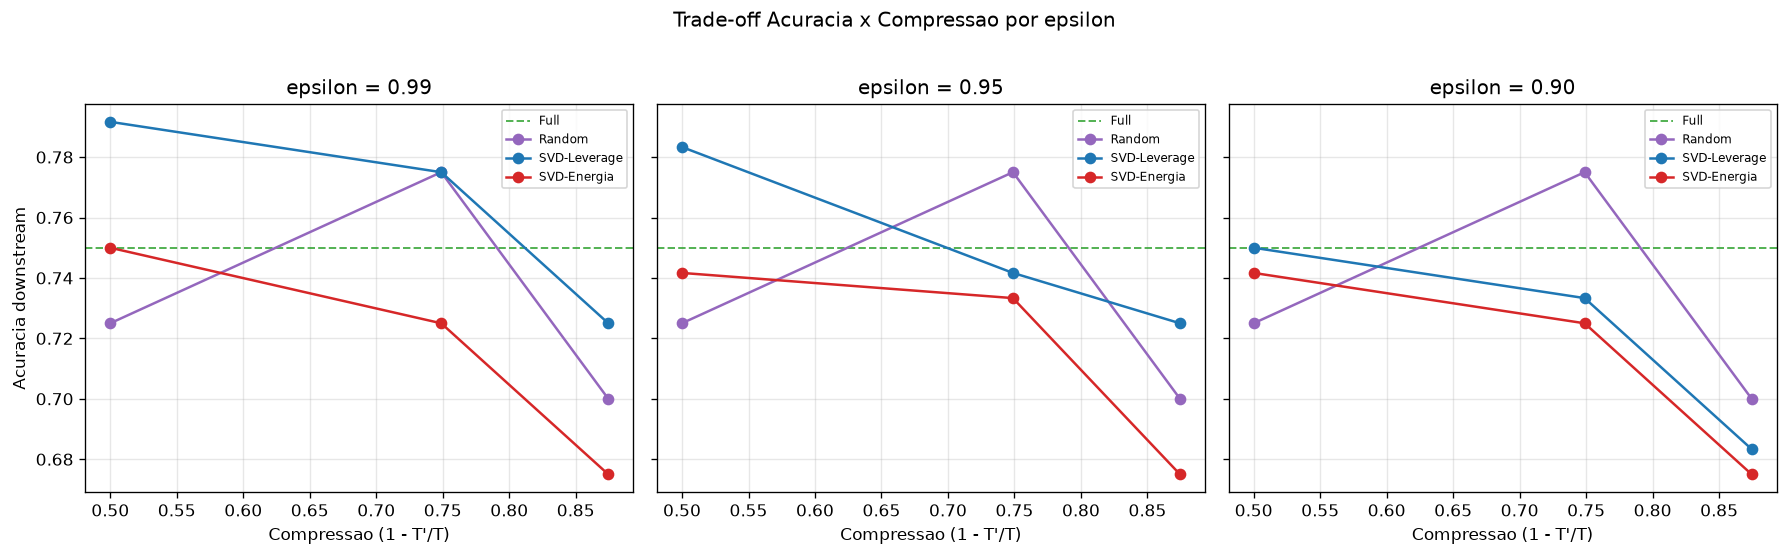
\includegraphics[width=\linewidth]{figures/tradeoff_acerto_compressao.png}
    \caption{Acurácia downstream $\times$ compressão (IMDb), facetada por $\varepsilon$. Cada painel compara os quatro métodos nos três níveis de $\rho$.}
    \label{fig:tradeoff}
\end{figure}

\begin{table}[ht]
    \centering
    \caption{Acurácia downstream por método e $\rho$ com $\varepsilon=0{,}90$.}
    \label{tab:imdb-e90}
    \small
    \begin{tabular}{lccc}
        \hline
        Método & $\rho=0{,}50$ & $\rho=0{,}25$ & $\rho=0{,}125$ \\
        \hline
        full & 0,750 & 0,750 & 0,750 \\
        random & 0,725 & 0,775 & 0,700 \\
        svd & 0,750 & 0,733 & 0,683 \\
        svd\_energia & 0,742 & 0,725 & 0,675 \\
        \hline
    \end{tabular}
\end{table}

\begin{table}[ht]
    \centering
    \caption{Acurácia downstream por método e $\rho$ com $\varepsilon=0{,}95$.}
    \label{tab:imdb-e95}
    \small
    \begin{tabular}{lccc}
        \hline
        Método & $\rho=0{,}50$ & $\rho=0{,}25$ & $\rho=0{,}125$ \\
        \hline
        full & 0,750 & 0,750 & 0,750 \\
        random & 0,725 & 0,775 & 0,700 \\
        svd & 0,783 & 0,742 & 0,725 \\
        svd\_energia & 0,742 & 0,733 & 0,675 \\
        \hline
    \end{tabular}
\end{table}

\begin{table}[ht]
    \centering
    \caption{Acurácia downstream por método e $\rho$ com $\varepsilon=0{,}99$.}
    \label{tab:imdb-e99}
    \small
    \begin{tabular}{lccc}
        \hline
        Método & $\rho=0{,}50$ & $\rho=0{,}25$ & $\rho=0{,}125$ \\
        \hline
        full & 0,750 & 0,750 & 0,750 \\
        random & 0,725 & 0,775 & 0,700 \\
        svd & 0,792 & 0,775 & 0,725 \\
        svd\_energia & 0,750 & 0,725 & 0,675 \\
        \hline
    \end{tabular}
\end{table}

\subsection{Pooling médio e poda moderada}\label{sec:pooling-poda}

Em $\rho=0{,}50$ e $\varepsilon=0{,}99$, \texttt{svd} supera levemente \texttt{full} (0,792 vs.\ 0,750; Tabela~\ref{tab:imdb-e99}). Não interpretamos isso como generalização \emph{cross-corpus}: a SVD é por documento e não supervisionada. A hipótese mais plausível, dado o protocolo de avaliação (Seção~\ref{sec:protocolo-clf}), é que a \textbf{poda melhore o pooling médio} usado como representação da review.

Com \texttt{full}, agregamos $\bar{T}\approx 209$ linhas de $F$ por média aritmética antes da normalização $L_2$ e do Ridge. Em reviews longas e redundantes, muitos subtokens contribuem pouco ao subespaço dominante da matriz --- enredo, repetições, trechos neutros --- mas entram com peso igual no pooling, \textbf{diluindo} o vetor agregado em $\mathbb{R}^D$. Com \texttt{svd} em $\rho=0{,}50$, mantêm-se $\bar{T'}\approx 105$ linhas ranqueadas por leverage no subespaço $F_k$; tokens de alta participação estrutural passam a pesar mais na média \emph{por exclusão} dos demais, produzindo um embedding de documento potencialmente mais \textbf{concentrado} para a tarefa de sentimento.

Dois elementos modulam essa leitura. Primeiro, o ganho de \texttt{svd} sobre \texttt{full} em $\rho=0{,}50$ só aparece claramente quando $\varepsilon$ é alto (0,750 em $\varepsilon=0{,}90$; 0,792 em $\varepsilon=0{,}99$): um subespaço $F_k$ mais rico ($\bar{k}\approx 92$) refina o ranqueamento antes da poda. Segundo, \texttt{random} também supera \texttt{full} em $\rho=0{,}25$ (0,775), o que indica que \textbf{reduzir o número de linhas agregadas} por si só pode ajudar neste proxy; o leverage acrescenta vantagem sobretudo em compressão mais agressiva ($\rho=0{,}125$) e quando $\varepsilon$ é elevado.
\subsection{Leitura algébrica dos métodos}

\texttt{svd} e \texttt{svd\_energia} compartilham a mesma decomposição singular, mas produzem rankings distintos:
\begin{itemize}
    \item \textbf{\texttt{svd}}: leverage clássico ($\ell_i/k$).
    \item \textbf{\texttt{svd\_energia}}: participação das linhas ponderada pelos valores singulares.
\end{itemize}
\texttt{svd\_energia} permanece abaixo de \texttt{svd} na maioria dos pares $(\varepsilon, \rho)$ e atinge 0,675 em $\rho=0{,}125$, independente de $\varepsilon$. Ponderar por $\Sigma_k$ concentra o ranking nos modos de maior energia; componentes menos dominantes podem ainda carregar sinal discriminativo para sentimento. Preservar energia espectral e preservar sinal downstream não coincidem necessariamente.

\subsection{Síntese dos achados}

Em relação às perguntas da Seção~\ref{sec:metodologia}:
\begin{enumerate}
    \item \textbf{Leverage score e acurácia}: a seleção por leverage mantém acurácia competitiva em compressão moderada; empata com \texttt{random} em $\rho=0{,}25$ (0,775) e supera em $\rho=0{,}125$ (0,725 vs.\ 0,700).
    \item \textbf{\texttt{svd\_energia} vs.\ \texttt{svd}}: a variante ponderada difere de \texttt{svd} e piora em $\rho$ baixo.
    \item \textbf{Invariância espectral a $\rho$}: $E_k^{\mathrm{energia}}$, $\bar{R}_k$ e $\bar{k}$ variam com $\varepsilon$ e permanecem invariantes a $\rho$ (Tabela~\ref{tab:metricas-eps}); medem $F_k$, não $S$.
\end{enumerate}

No proxy IMDb, $\varepsilon$ define o subespaço $F_k$, os leverage scores convertem esse subespaço em importância por token, e $\rho$ aplica a poda. A comparação com \texttt{svd\_energia} indica que maximizar energia espectral nos modos dominantes não coincide com maximizar utilidade supervisionada.
